
\documentclass[a4paper]{article}
\usepackage[OT1]{fontenc}
\usepackage{Sweave}
\usepackage[authoryear]{natbib}
\usepackage{fullpage}
\usepackage{amsmath}
\bibliographystyle{plainnat}

\DefineVerbatimEnvironment{Sinput}{Verbatim} {xleftmargin=2em}
\DefineVerbatimEnvironment{Soutput}{Verbatim}{xleftmargin=2em}
\DefineVerbatimEnvironment{Scode}{Verbatim}{xleftmargin=2em}
\fvset{listparameters={\setlength{\topsep}{0pt}}}
\renewenvironment{Schunk}{\vspace{\topsep}}{\vspace{\topsep}}

%%\VignetteIndexEntry{Capture-recapture}

\title{Capture-recapture models in {\tt unmarked}}
\author{Richard Chandler}


\begin{document}

\maketitle

\abstract{The ``{\tt un}'' in {\tt unmarked} is somewhat misleading
  because the package can be used to analyze data from marked animals. The three
  most common sampling methods that produce suitable data are removal
  sampling, double observer sampling, and capture-recapture
  methods\footnote{Sometimes animals are not actually marked when
    using these methods, but they are treated as though
    they are}. This document focuses on the analysis of capture-recapture
  data using a class of models known as multinomial $N$-mixture
  models \citep{royle_generalized_2004, fiskeChandler_2011}, which
  assume that capture-recapture data have been collected at a
  collection of sample locations (``sites''). Capture-recapture models
  can be fitted with
  constant parameters ($M_0$), time-specific parameters ($M_t$),
  and behavioral responses ($M_b$). In addition, spatial
  variation in abundance or capture probability can also be
  modeled using site-specific covariates. \pkg{unmarked} has two
  functions for fitting
  capture-recapture models: \code{multinomPois} and
  \code{gmultmix}. Both allow for user-defined functions to describe
  the capture process, and the latter allows for modeling of temporary
  emigration when data have been collected using the so-called robust
  design.
}


\section{Introduction}

In traditional capture-recapture models, $n$ individuals are captured
at a site during the course of $J$ sampling occasions. The encounter
history for each individual is used as information about capture
probability $p$ such that the total population size $N$ can be
regarded as the size parameter of a binomial distribution, $n \sim
\mbox{Binomial}(N, p)$. When capture probability is assumed to be
constant among individuals and over time, the model is refered to as
model $M_0$. Temporal variation in $p$ is assumed by the so-called
model $M_t$. Likewise, behavioral responses, such as trap-avoidance or
``trap-happiness'' can be modeled using model $M_b$.

Although traditional capture-recapture models represent the primary
method for estimating population size, they do not allow one to model
variation in abundance which is a central focus of much ecological
research.
\citet{royle_generalized_2004} developed a framework for
modeling variation in both abundance and capture
probability when capture-recapture data is collected at a set of
$R$ sites. Site-specific abundance ($N_i; i=1,2,...,R$) is regarded
as latent variable following a discrete distrubution such as the
Poisson or negative binomial. The encounter histories are then
tabulated at each site so that they can be regarded as an outcome of a
multinomial distribution with cell probabilities {$\bold \pi$}
determined by a protocol-specific function of capture
probability (see next section for details). Assuming a Poisson
distribution, the model can be written as
\begin{gather}
  N_i \sim \mbox{Poisson}(\lambda) \nonumber \\
  {\bf y_i}|N_i \sim \mbox{Multinomial}(N_i, \pi(p))
  \label{mod}
\end{gather}
In the above, $\lambda$ is the expected number of individuals at each
site. ${\bf y_i}$ is a vector containing the number of
individuals with encounter history $k; k=1,2,...K$ at site $i$. The
number of observable encounter histories $K$ depends on the sampling
protocol. For a capture-recapture study with 2 time periods, $K$
equals 3 because the possibilities are $(11, 10, 01)$. In Equation~\ref{mod},
$\pi(p)$ is a function that that converts capture probability $p$ to
multinomial cell probabilities, \emph{i.e.}, the proportion
of individuals expected to have capture history $k$. The definition of
$\pi(p)$ is also specific to the sampling protocol. For example, the
cell probabilities corresponding to the capture histories listed above
are
\[
{\bold \pi(p)} = \{p^2, p(1-p), (1-p)p, (1-p)^2\}.
\]
Note that the last multinomial cell probability corresponds to the
probability of not being captured.

Spatial variation in abundance can be modeled using covariates
with a log-link function
\[
\exp(\lambda_i) = \beta_0 + \beta_1 x_i
\]
where $x_i$ is some site-specific covariate such as habitat type or
elevation. Of course, multiple covariate effects can be consered an a
more general form of the above can be written as $\exp(\lambda_i) =
{\bf X_i' \beta}$ where ${\bf X}$ is a design matrix and ${\bf \beta}$ is a vector
of coefficients, possibly including an intercept.
Capture probability can be modeled in the same way using the logit
instead of the log link. For instance, we could have
\[
logit(p_{ij}) = \alpha_0 + \alpha_1 v_{ij}
\]
where $v_{ij}$ is some covariate specific to the site and
capture occasion.


\section{Data}
As previously mentioned, the data required by \pkg{unmarked} are an $R \times K$
matrix in which each row is the vector of tabulated encounter
histories for animals captured at some site. Capture-recapture data,
however, is typically recorded in the format shown in
Table~\ref{tab:raw}.

\begin{table}[h]
  \centering
  \caption{Capture-recapture data for 3 individuals. There were 3
    trapping occasions}
  \begin{tabular}{lcc}
    \hline
    Animal ID   & Site  & Capture history \\
    \hline
    GB        & A     & 101 \\
    YR        & A     & 101 \\
    RO        & A     & 111 \\
    PP        & A     & 100 \\
    GY        & B     & 100 \\
    PR        & B     & 010 \\
    \hline
  \end{tabular}
  \label{tab:raw}
\end{table}

In the absence of individual covariates, these data can be collapsed
and formatted as shown in Table~\ref{tab:format}. The \code{table}
function in \proglang{R} makes this conversion very easy, as
demonstrated in the next section.

\begin{table}[h]
  \centering
  \caption{Capture-recapture data from Table~\ref{tab:raw} in the
    format required by \pkg{unmarked}. Note that no animals were
    captured in sites C or D.}
  \begin{tabular}{lccccccc}
    \hline
    Site  & 100 & 010 & 001 & 110 & 011 & 101 & 111 \\
    \hline
    A     & 1   & 0   & 0   & 0   & 0   & 2   & 1   \\
    B     & 1   & 1   & 0   & 0   & 0   & 0   & 0   \\
    C     & 0   & 0   & 0   & 0   & 0   & 0   & 0   \\
    D     & 0   & 0   & 0   & 0   & 0   & 0   & 0   \\
    \hline
  \end{tabular}
  \label{tab:format}
\end{table}







\section{Analysis in \pkg{unmarked}}




\subsection{Closed population capture-recapture models}


In this example we will analyze point count data collected on the Alder
Flycatcher (\emph{Empidonax alnorum}) by
\citet{chandler_etal:2009}. Point count data such as these are
collected on unmarked animals, but one can apply
capture-recapture models because it is possible to keep track of
inidividual birds during a short period of time. That is, we can
pretend like birds are marked by noting which time intervals they are
detected in during a short survey. The alder flycatcher data were
collected using a 15-minute point counts, which were divided into 3
5-minute intervals. Thus, the ``capture history'' for a bird detected
in all 3 intervals would be ``111''. The following command imports the
capture histories for 50 individuals detected in 2005 at 49 point
count locations. Note that each point was surveyed three times. To
simply the analysis we first subset the data to work with the data
from the first visit.

\begin{Schunk}
\begin{Sinput}
> alfl <- read.csv(system.file("csv", "alfl.csv", package="unmarked"))
> head(alfl, 5)
\end{Sinput}
\begin{Soutput}
         id survey interval1 interval2 interval3
1 crick1_05      1         1         1         1
2 crick1_05      3         1         0         1
3   his1_05      1         0         1         1
4   his1_05      1         1         1         1
5   his1_05      2         0         1         1
\end{Soutput}
\end{Schunk}

We see 5 rows of data representing the encounter histories for 5 birds
detected at 2 points during 3 survey occasions. From these 5 birds, it appears as though
detection probability is high since each bird was detected during at
least 2 of the three time intervals.

Associated with the bird data are site- and visit-specific covariates
for each of the 49 sites. We can import these data using the following
command:

\begin{Schunk}
\begin{Sinput}
> alfl.covs <- read.csv(system.file("csv", "alflCovs.csv", package="unmarked"),
                          row.names=1)
> head(alfl.covs)
\end{Sinput}
\begin{Soutput}
          struct woody time.1 time.2 time.3 date.1 date.2 date.3
crick1_05   5.45  0.30   8.68   8.73   5.72      6     25     34
his1_05     4.75  0.05   9.43   7.40   7.58     20     32     54
hisw1_05   14.70  0.35   8.25   6.70   7.62     20     32     47
hisw2_05    5.05  0.30   7.77   6.23   7.17     20     32     47
kenc1_05    4.15  0.10   9.57   9.55   5.73      8     27     36
kenc2_05    9.75  0.40   9.10   9.12   9.12      8     27     36
\end{Soutput}
\end{Schunk}

Each row of this \code{data.frame} corresponds to a point count
location. The variable \code{struct} is a measure of vegetation
structure, and \code{woody} is the percent cover of woody vegetation
at each of the 50-m radius plots. Time of day and date were measured
for each of the three visits.

To format the data for \pkg{unmarked}, we need to tabulate the
encounter histories for each site. Before doing so, let's first put
our capture histories in a single column. Let's also be explicit about
the levels of our factors for both the newly created captureHistory
column and the point id column

\begin{Schunk}
\begin{Sinput}
> alfl$captureHistory <- paste(alfl$interval1, alfl$interval2, alfl$interval3, sep="")
> alfl$captureHistory <- factor(alfl$captureHistory,
     levels=c("001", "010", "011", "100", "101", "110", "111"))
> ## NOOOOOOO
> #levels(alfl$id) <- rownames(alfl.covs)
> alfl$id <- factor(alfl$id, levels=rownames(alfl.covs))
\end{Sinput}
\end{Schunk}

Setting the levels of \code{captureHistory} ensures that when we
tabulate the encounter histories, we will include zeros for histories
that were not observed. Similarly, setting the levels of
\code{alfl\$id} tells \proglang{R} that there
were some sites where no ALFL were detected. This way, when we
tabulate the data, we get a frequency for each site, not just the ones
with $>1$ detection. Let's go ahead and tabulate the encounter
histories for the first survey occasion.

\begin{Schunk}
\begin{Sinput}
> alfl.v1 <- alfl[alfl$survey==1,]
> alfl.H1 <- table(alfl.v1$id, alfl.v1$captureHistory)
> head(alfl.H1, 5)
\end{Sinput}
\begin{Soutput}
            001 010 011 100 101 110 111
  crick1_05   0   0   0   0   0   0   1
  his1_05     0   0   1   0   0   0   1
  hisw1_05    0   0   0   0   0   0   0
  hisw2_05    0   0   0   0   0   0   1
  kenc1_05    0   0   0   0   0   0   0
\end{Soutput}
\end{Schunk}

The object \code{alfl.H1} contains the tabulated capture histories for
each site. This is the format required by unmarked. Note that this
data also suggests that detection probability was high since the most
common encounter history (for these 5 points) was $111$. Note also that
no birds were detected at point \code{hisw1\_05}.

Now we are almost ready to create our \code{unmarkedFrame} and begin
fitting models. We will fit our first series of models using the
\code{multinomPois} function, which requires data formated using the
\code{unmarkedFrameMPois} function. This constructor function
recognizes two types of capture-recapture data: removal sampling
data and double observer sampling data. In the future, we may add an
option to automatically handle standard capture-recapture data too,
but here we show how to supply it using a user-defined \code{piFun},
which allows extreme flexibility in converting detection probability
to multinomial cell probabilities $\bold \pi$. The \code{piFun} must
take a matrix of detection probabilities with as many columns as there
are columns of $\bf y$, and convert them to a matrix of multinomial
cell probabilities with $K$ columns. Each column corresponds to the
probability of observing the encounter history $k$. Here is a
\code{piFun} to compute the multinomial cell probabilities when there
were 3 sampling occasions. Note that the probabilities are simply $p$
for a detection and $1-p$ for a non-detection.

\begin{Schunk}
\begin{Sinput}
> crPiFun <- function(p) { # p should have 3 columns
     cbind("001" = (1-p[,1]) * (1-p[,2]) * p[,3],
           "010" = (1-p[,1]) * p[,2]     * (1-p[,3]),
           "011" = (1-p[,1]) * p[,2]     * p[,3],
           "100" = p[,1]     * (1-p[,2]) * (1-p[,3]),
           "101" = p[,1]     * (1-p[,2]) * p[,3],
           "110" = p[,1]     * p[,2]     * (1-p[,3]),
           "111" = p[,1]     * p[,2]     * p[,3])
 }
\end{Sinput}
\end{Schunk}

To demonstrate how this works, imagine that we surveyed 2 sites and
detection probability was constant ($p=0.2$) among sites and survey
occasions. The function converts these capture probabilities to
multinomial cell probabilites. Note that these cell probabilites will
sum to $< 1$ if capture probability less than 1 over the 3 occasions.

\begin{Schunk}
\begin{Sinput}
> p <- matrix(0.4, 2, 3)
> crPiFun(p)
\end{Sinput}
\begin{Soutput}
       001   010   011   100   101   110   111
[1,] 0.144 0.144 0.096 0.144 0.096 0.096 0.064
[2,] 0.144 0.144 0.096 0.144 0.096 0.096 0.064
\end{Soutput}
\begin{Sinput}
> rowSums(crPiFun(p))
\end{Sinput}
\begin{Soutput}
[1] 0.784 0.784
\end{Soutput}
\end{Schunk}





obsToY needs to be a matrix with
the number of rows equal to the number of columns for some obsCov, and
the number columns equal to the number of columns in y
If obsToY[i,j] is 1, then a missing value in obsCov translates to
a missing value in y. For capture-recapture data, all elements of
\code{obsToY} should be 1.

\begin{Schunk}
\begin{Sinput}
> o2y <- matrix(1, 3, 7)
\end{Sinput}
\end{Schunk}



\begin{Schunk}
\begin{Sinput}
> library(unmarked)
> intervalMat <- matrix(c('1','2','3'), 50, 3, byrow=TRUE)
> class(alfl.H1) <- "matrix"
> umf.cr1 <- unmarkedFrameMPois(y=alfl.H1,
                         siteCovs=alfl.covs[,c("woody", "struct", "time.1")],
                         obsCovs=list(interval=intervalMat),
                         obsToY=o2y, piFun="crPiFun")
\end{Sinput}
\end{Schunk}


Writing a \code{piFun} and creating the \code{obsToY} object are
the hardest parts of a capture-recapture analysis in
\pkg{unmarked}. Again, this is done automatically for removal models
and double observer models, and we may add an option to do this
automatically for capture-recapture data too, but hopefully it is
evident the flexibility allowed by specifying user-defined
functions. For example \code{crPiFun} could easily be modified to
allow for behavioral responses (trap-shyness) or for non-constant time
intervals.

Now that we have our data formatted we can fit some models. The
following correspond to model $M_0$, model $M_t$, and a model with a
continous covariate effect on $p$.


\begin{Schunk}
\begin{Sinput}
> M0 <- multinomPois(~1 ~1, umf.cr1)
> Mt <- multinomPois(~interval-1 ~1, umf.cr1)
> Mc <- multinomPois(~time.1 ~1, umf.cr1)
\end{Sinput}
\end{Schunk}

These sort of models can be fit in other software programs. What is
unique about \pkg{unmarked} is that we can also model variation in
abundance among sites. The following model treats abundance as
a function of the percent cover of woody vegetation.

\begin{Schunk}
\begin{Sinput}
> (M0.woody <- multinomPois(~1 ~woody, umf.cr1))
\end{Sinput}
\begin{Soutput}
Call:
multinomPois(formula = ~1 ~ woody, data = umf.cr1)

Abundance:
            Estimate    SE     z  P(>|z|)
(Intercept)   -0.962 0.325 -2.96 0.003059
woody          2.587 0.680  3.80 0.000143

Detection:
 Estimate    SE    z  P(>|z|)
     1.43 0.216 6.63 3.42e-11

AIC: 245.9301 
\end{Soutput}
\end{Schunk}


This final model has a much lower AIC score than the other models, and
it indicates
that ALFL abundance increases with the percent cover
of woody vegetation. We can plot this relationship by predicting
abundance at a sequence of woody vegetation values.

\begin{Schunk}
\begin{Sinput}
> nd <- data.frame(woody=seq(0, 0.8, length=50))
> E.abundance <- predict(M0.woody, type="state", newdata=nd, appendData=TRUE)
> plot(Predicted ~ woody, E.abundance, type="l", ylim=c(0, 6),
      ylab="Alder flycatchers / plot", xlab="Woody vegetation cover")
> lines(lower ~ woody, E.abundance, col=gray(0.7))
> lines(upper ~ woody, E.abundance, col=gray(0.7))
\end{Sinput}
\end{Schunk}
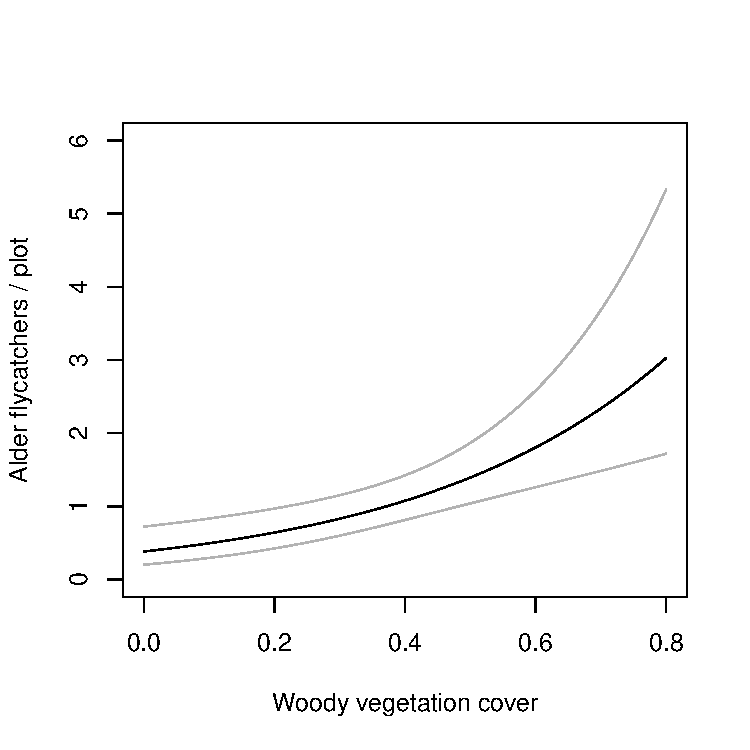
\includegraphics{cap-recap-012}


\section{Capture-recapture models allowing for temporary emigration}

In the previous analysis we used data from the first visit only.
\citet{chandlerEA_2011} proposed a model that allows us to
make use of the entire alder flycatcher dataset. The model is similar
to the temporary emigration model of \citet{kendall_etal:1997} except
that we are
interested in modeling variation in abundance among sites.

The model assumes that no births or deaths occur during the study
period, but animals may move on and off the plots between sampling
occasions. This type of movement is referred to as temporary
emigration. To account for it, define $M_$ to be the super-population
size, the total number of individuals that use site $i$ during the
study period. Assuming that we visit each site on $T$ occasions,
primary periods, define $N_{it}$ to be the subset of $M_i$ exposed
to sampling during occasion $t$. We now collect capture-recapture data
at each site during each primary period $t$, and obtain the data $\bf
y_{ijt}$. The model can be written as

\begin{gather}
  M_i \sim \mbox{Poisson}(\lambda) \nonumber \\
  N_{it} \sim \mbox{Binomial}(M_i, \phi) \\
  {\bf y_{it}}|N_{it} \sim \mbox{Multinomial}(N_{it}, \pi(p))
  \label{mod:te}
\end{gather}


The data structure for the robust design is more complex than before,
but it is easy to create in \proglang{R}. We can once again use the
\code{table} function---but this time, we create a three-dimensional table
rather than a two-dimensional one. We also need to expand the
\code{obsToY} mapping matrix. This isn't so intuitive, but the
commands below are generic and can be applied to other
capture-recapture designs.

\begin{Schunk}
\begin{Sinput}
> alfl.H <- table(alfl$id, alfl$captureHistory, alfl$survey)
> alfl.Hmat <- cbind(alfl.H[,,1], alfl.H[,,2], alfl.H[,,3])
> nVisits <- 3
> o2yGMM <- kronecker(diag(nVisits), o2y)
> umf.cr <- unmarkedFrameGMM(y=alfl.Hmat,
     siteCovs=alfl.covs[,c("woody", "struct")],
     yearlySiteCovs=list(date=alfl.covs[,3:5],
                         time=alfl.covs[,6:8]),
     obsCovs=list(interval=cbind(intervalMat,intervalMat,intervalMat)),
     obsToY=o2yGMM, piFun="crPiFun", numPrimary=nVisits)
\end{Sinput}
\end{Schunk}


Notice that we have 3 types of covariates now. The site-specific
covariates are the same as before. Now, however, the observation
covariates must match the dimensions of the {\bf y} matrix. We can
also have a class of covariates that vary among primary periods but
not within primary periods. These are called yearlySiteCovs, which is
a misleading name. It is a carry-over from other ``open population"
models in \pkg{unmarked}, but it should be remembered that these
models are most suitable for data from a single year, since we assume
no births or mortalities.

We can fit the model using the \code{gmultmix} function, which has a
slightly different set of arguments. Rather than a single formula, the
function takes 3 formulas for abundance covariates, availability
covariates, and detection covariates in that order.


\begin{Schunk}
\begin{Sinput}
> (fm1 <- gmultmix(~woody, ~1, ~time+scale(date), umf.cr))
\end{Sinput}
\begin{Soutput}
Call:
gmultmix(lambdaformula = ~woody, phiformula = ~1, pformula = ~time + 
    scale(date), data = umf.cr)

Abundance:
            Estimate    SE      z P(>|z|)
(Intercept)  -0.0897 0.393 -0.228 0.81944
woody         2.4294 0.591  4.107 0.00004

Availability:
 Estimate    SE     z P(>|z|)
   -0.782 0.495 -1.58   0.114

Detection:
            Estimate     SE      z  P(>|z|)
(Intercept)   1.8900 0.2998  6.304 2.91e-10
time         -0.0499 0.0142 -3.526 4.22e-04
scale(date)  -0.0362 0.1740 -0.208 8.35e-01

AIC: 580.4508 
\end{Soutput}
\end{Schunk}

Results from this model are similar to those obtained using the subset
of data, but the standard error for the woody estimate has decreased.


\section{Individual Heteogeneity in Capture Probability}

The capture-recapture models that can be fit in \pkg{unmarked} assume
that variation in capture probability can be
explained by site, time, or behavioral factors. Individual
heterogeneity cannot be explicitly modeled, although, one could
partition the data into strata and analyze the strata separately. For
example, sex-specific
differences could be studied by dividing the data into 2 subsets.
Continuous animal-specific covariates, however, cannot be
considered in \pkg{unmarked}. The so-called model $M_h$, which assumes
random variation in capture probability among individuals is also not
allowed. Some might find comfort in this given the concerns about
$M_h$ raised by \citet{link:2003}.

Another source of individual heterogeneity in capture probability
arises from the distance between an individual's area of activity and
the trap location. Traditional capture-recapture models ignore this
important source of variation in capture probability, but
recently developed spatial capture-recapture models overcome this
limitation. SCR models also yield estimates of density rather than
just population size, which is important when the study area cannot be
well-defined. See xyz for
more information.

Spatial capture-recapture models would not work well with the alder
flycatcher data because they require ``spatial recaptures''. That is,
the models work best when individuals are encountered at multiple
locations. We also do not see any reason to worry about
distance-related heterogeneity in detection for this dataset because
the sample plots were so small (0.785 ha) and we analyzed data from
singing individuals only.

\bibliography{unmarked}



\end{document}
